\section{Aufbau und Kernmerkmale von MP4-Containern}
\label{kap:aufbau_mp4}

Das MP4-Dateiformat ist ein standardisiertes Multimedia-Containerformat, dessen formale Spezifikation in der Norm ISO/IEC 14496-14 definiert ist \cite{iso_14496-14_2020}. Es baut architektonisch auf dem ISO Base Media File Format (ISOBMFF) gemäß ISO/IEC 14496-12 auf, welches wiederum seine historischen Wurzeln im objektorientierten Apple-QuickTime-Format hat \cite{apple_quicktime_2001}. 

%%%

\subsection{Formale Spezifikation und Nomenklatur}

Die Architektur eines MP4-Containers ist streng hierarchisch als Baumstruktur aufgebaut. Die elementaren Strukturen dieser Topologie werden im ISO-Standard formal als \textit{Boxen} bezeichnet, während in der älteren QuickTime-Spezifikation und in Teilen der forensischen Literatur synonym der Begriff \textit{Atom} verwendet wird \cite{iso_14496-12_2022}. In der vorliegenden Arbeit wird der standardkonforme Begriff der Box verwendet. \\

TODO: Kurzer Absatz, was welche Norm genau definiert und sich somit voneinander abgrenzen\\

TODO: Übersicht/Grafik der Normanen mit den relevantesten Boxen, die diese definieren\\

Jede Box ist syntaktisch strikt definiert und beginnt zwingend mit einem Header. Dieser Header enthält die Bytegröße der Box sowie einen eindeutigen Vier-Zeichen-Code (Four-Character Code oder kurz 4CC), der den Typ und damit die semantische Bedeutung des Datenblocks definiert (z.\,B. \(ftyp\), \(moov\), \(mdat\)). Abhängig von ihrem Typ können Boxen als reine Containerstrukturen fungieren, die wiederum weitere Unter-Boxen aufnehmen, oder als sogenannte Leafs (Blätter), die ausschließlich isolierte Metadaten oder binäre Parameter enthalten \cite[Kap. 4]{iso_14496-12_2022}.

%%%

\subsection{Funktionale Trennung von Metadaten und Bitstrom}

Ein Kernmerkmal des ISOBMFF ist die funktionale und physische Trennung zwischen den strukturellen Metadaten und dem eigentlichen audiovisuellen Bitstrom. Diese Trennung ermöglicht es, die Topologie der Datei zu analysieren, ohne den rechenintensiven Videostream dekodieren zu müssen \cite[S. s69]{gloe_forensic_2014}.\\

TODO: Grafik aus ISO erweitern \cite[Figure A1.]{iso_14496-12_2022}

\begin{figure}
    \centering
    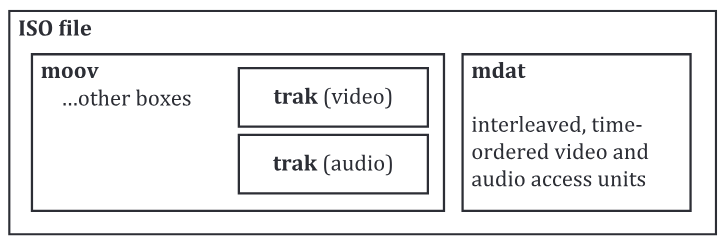
\includegraphics[width=0.8\linewidth]{grafiken/mp4-trak.png}
    \caption{TODO: mp4-trak.png \cite[Figure A1.]{iso_14496-12_2022}}
    \label{fig:mp4trak}
\end{figure}

Die Metadaten, die alle Verknüpfungen, Timing-Informationen und Codec-Konfigurationen umfassen, werden zentral in der \(moov\)-Box (Movie Box) gespeichert. Diese fungiert als Top-Level-Container für den gesamten Metadaten-Baum und enthält unter anderem die \(trak\)-Boxen (siehe \cref{fig:mp4trak}), welche die Konfigurationen für die individuellen Medienspuren definieren \cite[Kap. 8.2]{iso_14496-12_2022}. Im Gegensatz dazu speichert die \(mdat\)-Box (Media Data Box) die rohen, komprimierten Audio- und Videodaten. Da die \(mdat\)-Box in der Regel den Großteil der Dateigröße beansprucht, intern jedoch keine ISO-konformen Unterstrukturen mehr aufweist, wird sie für die strukturelle Container-Forensik in der Regel als Blackbox betrachtet und von der syntaktischen Analyse exkludiert \cite[Kap. 8.1]{iso_14496-12_2022}.

%%%

\subsection{Herstellerspezifische Syntaktik und proprietäre Erweiterungen}

Obwohl der ISO-Standard die grundlegende Topologie diktiert, gewährt er Software-Encodern, Kameraherstellern und zunehmend auch KI-Video-Generatoren erhebliche Freiheitsgrade bei der Anordnung und Nutzung optionaler Boxen \cite[S. s71]{gloe_forensic_2014}. 

Von besonderer forensischer Relevanz sind hierbei herstellerspezifische Erweiterungen (wie z.\,B. \(udta\) für User Data) sowie die explizit als Blanko-Container spezifizierte \(uuid\)-Box \cite[Kap. 8.2]{iso_14496-12_2022}. Die \(uuid\)-Box wird in der Praxis häufig genutzt, um proprietäre Metadaten oder kryptografische Signaturen (beispielsweise nach C2PA-Standard) zu implementieren. Die Existenz, die Dateigröße und die exakte Position dieser optionalen Boxen im MP4-Baum variieren stark zwischen verschiedenen Erzeugerquellen. Eben diese syntaktischen Abweichungen und herstellerspezifischen Nutzungsmuster bilden das fundamentale Merkmalset, welches im Rahmen dieser Arbeit für das Similarity Hashing extrahiert und quantifiziert werden soll \cite[S. s75]{gloe_forensic_2014}.

%%%

\subsection{Topologie und Exemplarischer Strukturbaum}

Zur Veranschaulichung der in den vorigen Abschnitten dargelegten Strukturprinzipien wird nachfolgend der Aufbau der Boxen einer standardkonformen MP4-Datei exemplarisch visualisiert. Dieses generische Beispiel illustriert sowohl die lineare Abfolge der Boxen auf der obersten Ebene als auch die tiefe Verschachtelung innerhalb des Metadaten-Containers \cite[Kap. 8]{iso_14496-12_2022}.\\

TODO: Grafik schöner machen\\

In einer typischen sequenziellen Anordnung (siehe \cref{fig:mp4-2}) steht die Kompatibilitätsdeklaration (\(ftyp\)) an erster Stelle, um dem Parser das primäre Dateiprofil zu signalisieren. Ihr folgt die Metadaten-Struktur (\(moov\)), bevor die eigentlichen Mediainhalte (\(mdat\)) den Hauptteil der Datei einnehmen \cite[S. s69]{gloe_forensic_2014}. 

\begin{figure}[H]
    \centering
    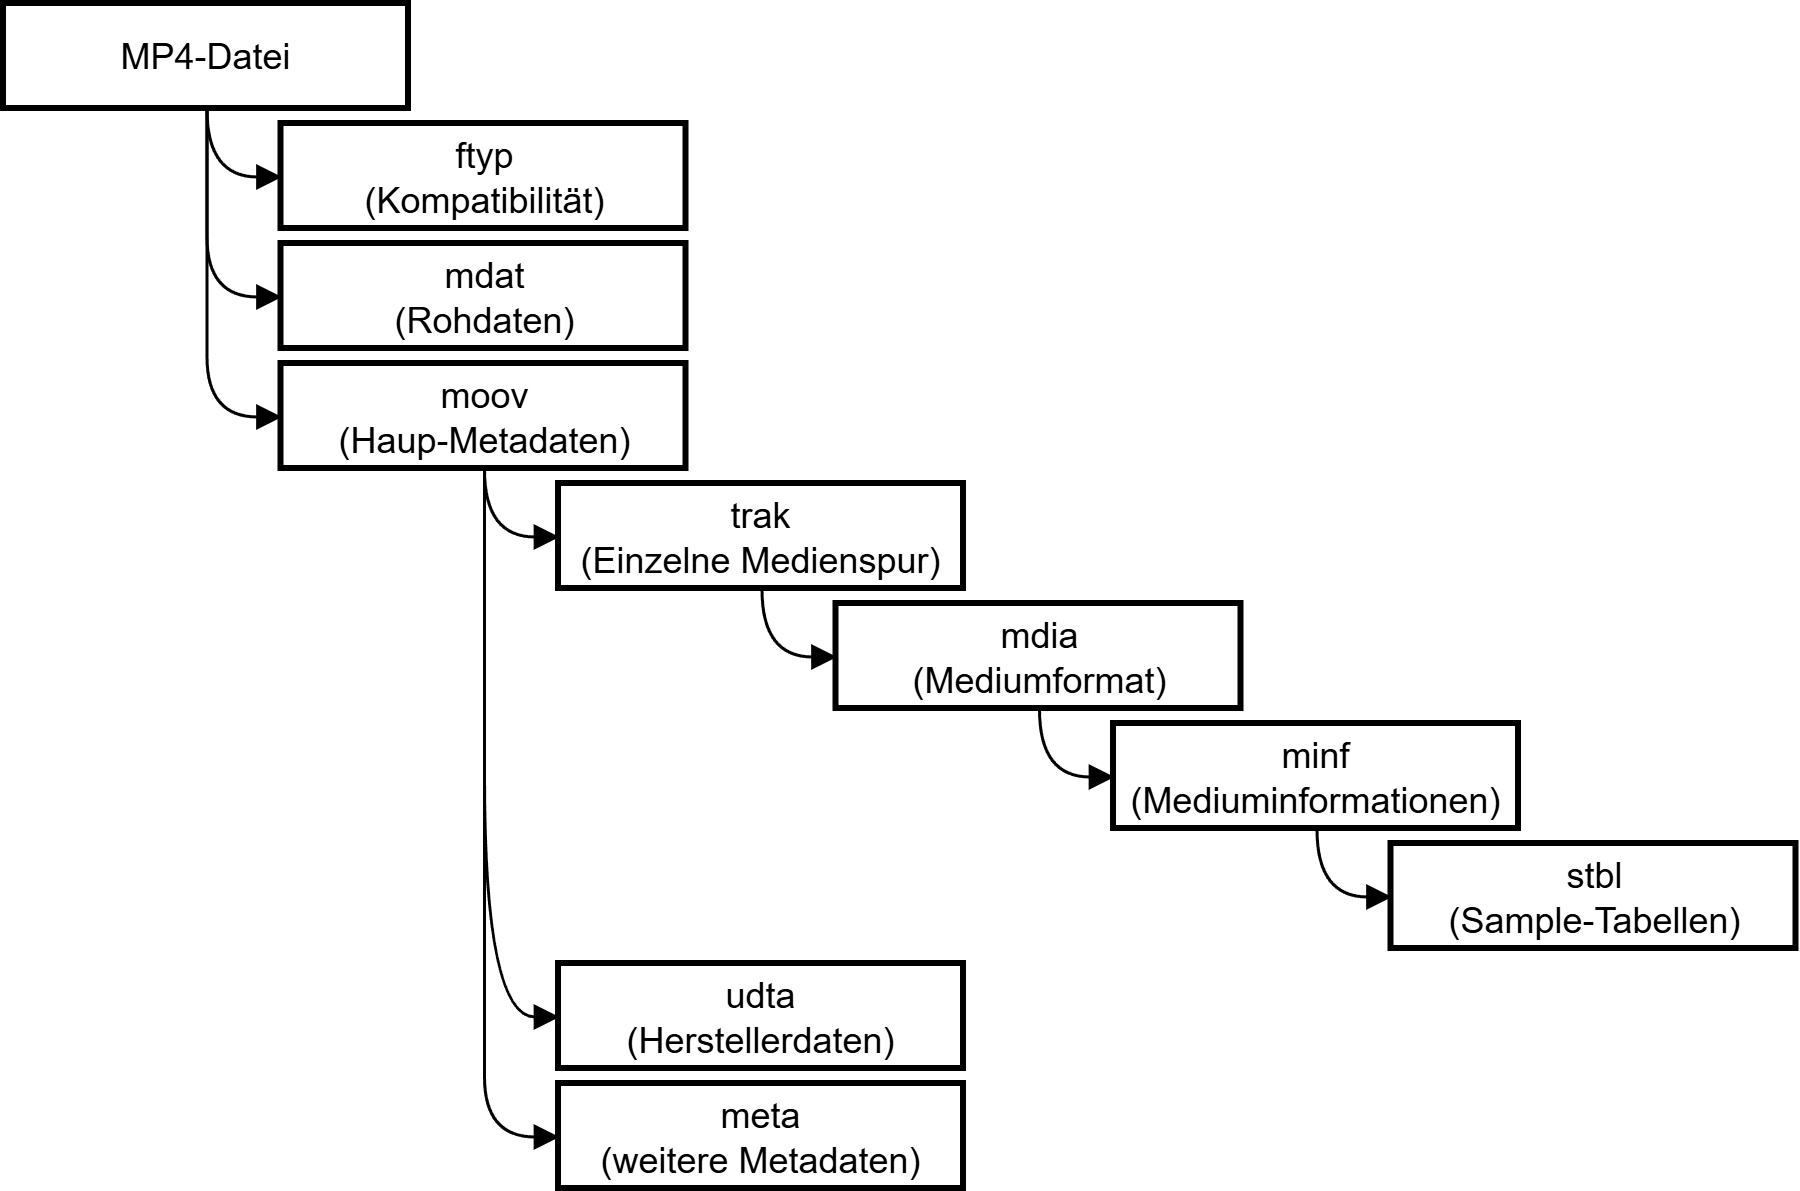
\includegraphics[width=0.8\linewidth]{grafiken/mp4-2.drawio.png}
    \caption{TODO: mp4-2.drawio}
    \label{fig:mp4-2}
\end{figure}

Anhand dieser Hierarchie wird ersichtlich, dass untergeordnete Blätter (Leafs) wie die \(stbl\)-Box erst durch ihren eindeutigen, absoluten Pfad (\(moov/trak/mdia/minf/stbl\)) im Gesamtkontext determinierbar sind. Weicht eine Software von dieser Standardtopologie ab, verschiebt sich die syntaktische Anordnung. Beispielsweise können die Metadaten am Dateiende (Fast-Start-Optimierung für Streaming) oder optionale \(uuid\)-Blöcke eingefügt werden.
